% ============================================================
%  OPTIMIZATION STRATEGY
% ============================================================


% ============================================================
\subsection{Transmutation Kinetics (D. Frank)}
\label{sec:transmutation-kinetics}
% ============================================================

The competition between plutonium production and destruction can be modeled through coupled Bateman equations. Assuming complete decay of $^{239}$Np to $^{239}$Pu ($t_{1/2} = 2.36$\,days, negligible relative to operational timescales), the transmutation dynamics reduce to:

\begin{align}
    \frac{dN_\text{U238}}{dt}  &\approx -\lambda_1 N_\text{U238}(t) \label{eq:U238-ode} \\
    \frac{dN_\text{Pu239}}{dt} &\approx \lambda_2 N_\text{U238}(t) - \lambda_3 N_\text{Pu239}(t) \label{eq:Pu239-ode}
\end{align}

\noindent where the flux-averaged microscopic reaction rates are:
\begin{equation}
    \lambda_1 = \Phi_0 \langle \sigma_\text{a,U238} \rangle, \qquad
    \lambda_2 = \Phi_0 \langle \sigma_{(n,\gamma),\text{U238}} \rangle, \qquad
    \lambda_3 = \Phi_0 \langle \sigma_\text{a,Pu239} \rangle
\end{equation}
with $\Phi_0$ the scalar neutron flux and $\langle \sigma_* \rangle$ denoting flux-averaged microscopic cross sections. Uranium-238 depletion follows exponential decay:
\begin{equation}
    N_\text{U238}(t) = N_\text{U238}(0)\,e^{-\lambda_1 t}
\end{equation}

Substituting into \eqref{eq:Pu239-ode} yields a first-order linear ODE. The necessary condition for net plutonium burning (a monotonically decreasing $^{239}$Pu inventory) requires:
\begin{equation}
    \lambda_3 N_\text{Pu239}(t) > \lambda_2 N_\text{U238}(0)\,e^{-\lambda_1 t} \qquad \forall\, t \geq 0
    \label{eq:burn-condition}
\end{equation}

This condition is most easily satisfied at $t = 0$ (beginning of life), where the right-hand side is at its maximum. It translates to a requirement on the ratio of the flux-averaged $^{239}$Pu absorption cross section to the $^{238}$U capture cross section:
\begin{equation}
    \frac{\lambda_3}{\lambda_2} = \frac{\langle \sigma_\text{a,Pu239} \rangle}{\langle \sigma_{(n,\gamma),\text{U238}} \rangle} \gg 1
    \label{eq:ratio-condition}
\end{equation}

Figure~\ref{fig:breed-burn-xs} shows the energy-dependent cross sections for both reactions. In the thermal energy range ($E \lesssim 1$\,eV), $\sigma_\text{a,Pu239}$ exceeds $\sigma_{(n,\gamma),\text{U238}}$ by two to three orders of magnitude, satisfying \eqref{eq:ratio-condition} and providing the driving physical rationale for heavy moderation. In the epithermal and fast regimes, the cross-section advantage of $^{239}$Pu diminishes substantially, making a softened neutron spectrum a prerequisite for achieving net plutonium burning.

\begin{figure}[H]
    \centering
    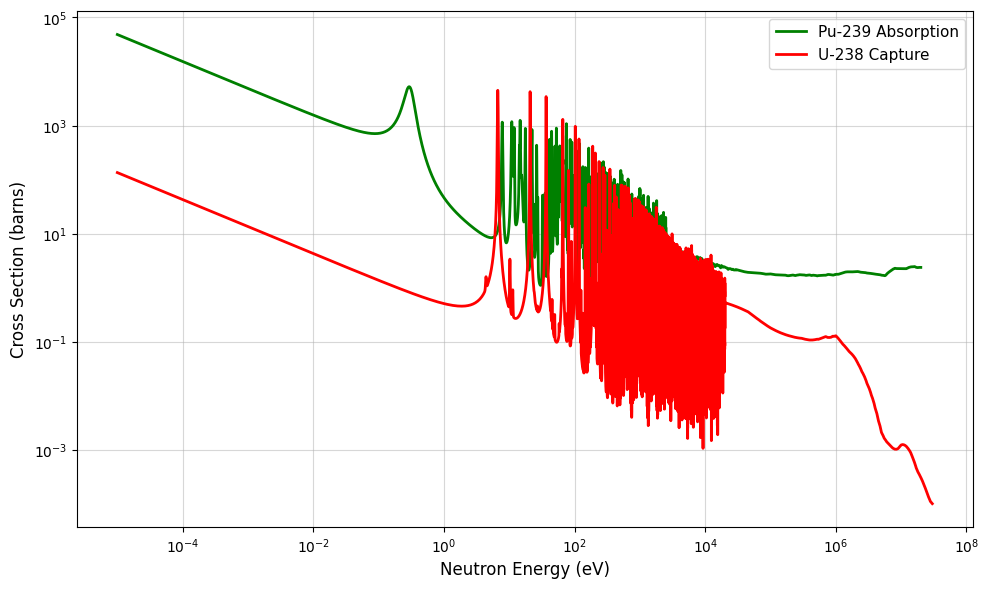
\includegraphics[width=0.75\linewidth]{figs/breed_burn_xs.png}
    \caption{Neutron cross sections for $^{238}$U radiative capture (breeding) and $^{239}$Pu absorption (burning) as functions of energy, evaluated from ENDF/B-VIII.0 at 900\,K \cite{Brown2018ENDF/B-VIII.0:Data}. In the thermal range, $\sigma_\text{a,Pu239}$ exceeds $\sigma_{(n,\gamma),\text{U238}}$ by two to three orders of magnitude, establishing the physical basis for the LBR's thermal spectrum strategy.}
    \label{fig:breed-burn-xs}
\end{figure}

% ============================================================
\subsection{Preliminary Neutronics Scoping (D. Frank)}
\label{sec:scoping}
% ============================================================

The cross-section analysis establishes the need for a highly thermalized spectrum but does not by itself determine the moderator material or lattice geometry. A series of preliminary scoping calculations was performed on an infinite lattice model to identify a viable design point before proceeding to higher-fidelity analysis.

\subsubsection{Moderator and Lattice Pitch: Infinite Lattice Study}

An infinite lattice model was constructed in OpenMC, selected for its seamless integration with Python scripting, which facilitated the parametric sweep over moderator types and lattice pitches. Fuel compositions were drawn from radiochemical assay data for a spent fuel rod at Three Mile Island Unit 1 (TMI-1|NJ05|H6|C2B), with a discharge burnup of 52.6\,GWd/tHM and an initial enrichment of 4.01\,wt\%. This sample, among the highest-burnup specimens in the SFCOMPO-2.0 database \cite{Michel-Sendis2017SFCOMPO-2.0:Data}, was selected as a conservative baseline on the basis that highly depleted fuel maximizes the challenge to criticality (see Appendix \ref{sec:app_fuel-ref}, Table \ref{tab:tmi1_rod_characteristics} for isotopic profile). Three moderator candidates were evaluated --- light water (H$_2$O), heavy water (D$_2$O), and helium --- over a lattice pitch range of 1.5 to 15\,cm.

Figure~\ref{fig:kinf-pitch} shows $k_\infty$ at startup as a function of lattice pitch for each moderator. Light water and helium fail to sustain criticality at any pitch for fuel of this burnup. Heavy water is the only candidate that achieves $k_\infty > 1$, owing to its low thermal neutron absorption cross section ($\sigma_\text{a,D2O} \approx 0.001$\,b) compared to light water ($\sigma_\text{a,H2O} \approx 0.33$\,b), which preserves neutron economy in a fuel-poor lattice. The D$_2$O system reaches $k_\infty > 1$ for pitches above $\sim$3\,cm and plateaus near 1.27 for pitches of 6 to 15\,cm.

\begin{figure}[H]
    \centering
    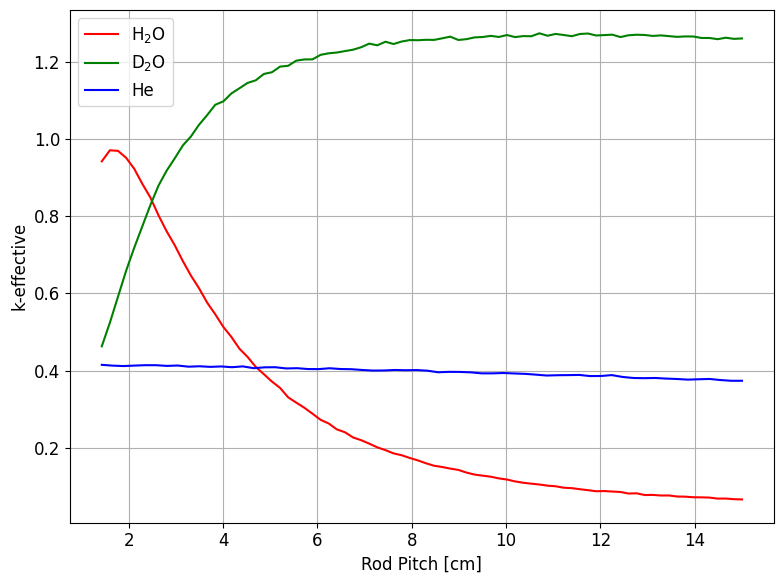
\includegraphics[width=0.73\linewidth]{figs/KinfVsPitch.png}
    \caption{Infinite multiplication factor $k_\infty$ at startup versus lattice pitch for H$_2$O, D$_2$O, and He moderation, using the TMI-1 spent fuel composition (52.6\,GWd/tHM). Light water and helium fail to achieve criticality at any pitch; D$_2$O reaches $k_\infty > 1$ for pitches above $\sim$3\,cm and plateaus near 1.27 for pitches of 6 to 15\,cm.}
    \label{fig:kinf-pitch}
\end{figure}

The reaction rates for $^{239}$Pu absorption (burning) and $^{238}$U capture (breeding) as functions of lattice pitch are compared in Figure~\ref{fig:breed-burn-rr}. Only the D$_2$O system satisfies the burning-over-breeding condition ($\lambda_3 > \lambda_2$) established in Section~\ref{sec:transmutation-kinetics}, and does so across a broad range of pitches, confirming heavy water as the only viable moderator for net plutonium reduction.

\begin{figure}[H]
    \centering
    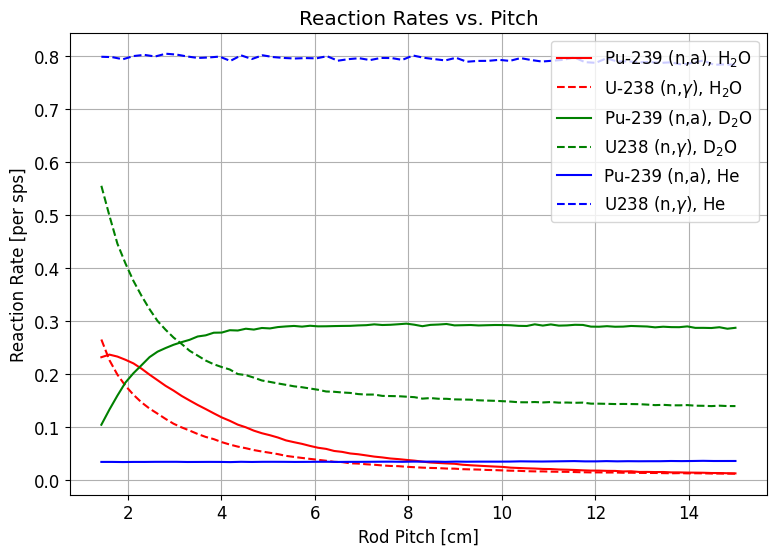
\includegraphics[width=0.73\linewidth]{figs/RRvsPitch.png}
    \caption{Normalized $^{239}$Pu absorption (burning) and $^{238}$U capture (breeding) reaction rates versus lattice pitch for H$_2$O and D$_2$O moderation. Heavy water uniquely sustains a configuration in which the burning rate exceeds the breeding rate ($\lambda_3 > \lambda_2$) over a broad pitch range, confirming D$_2$O as the only viable moderator for net plutonium reduction.}
    \label{fig:breed-burn-rr}
\end{figure}

A lattice pitch of 6\,cm was selected as the baseline design point, balancing three competing requirements:
\begin{enumerate}
    \item Sufficient spectrum thermalization to maintain $\lambda_3/\lambda_2 > 1$ (Objective~1: plutonium burning).
    \item Adequate initial excess reactivity ($k_\infty \approx 1.22$) to sustain criticality throughout the fuel cycle (Objective~2).
    \item Small enough to allow for sufficient heat removal (Objective~3), discussed further in \S~\ref{sec:th-scoping}. %FIND THIS
\end{enumerate}

\subsubsection{Zero-Dimensional Depletion Analysis}

Having established D$_2$O moderation at a 6\,cm pitch as the design point, a zero-dimensional (0-D) depletion analysis was performed to assess achievable burnup, plutonium burndown, and isotopic quality evolution under continuous irradiation at constant power. A specific power of 30\,W/gHM was assumed, consistent with typical PWR operation, yielding a total heavy metal inventory of approximately 67\,tonnes at 2\,GW$_\text{th}$ across $\sim$19,400 fuel rods.

\paragraph{Burnup Performance.}
Objective~2 requires $k_\text{eff} \geq 1$ through an accumulated discharge burnup of $\geq$60\,GWd/tHM. The 0-D model uses the TMI-1 C2B spent fuel composition (see App.~\ref{sec:app_fuel-ref}), which enters the LBR at 52.6\,GWd/tHM. The NRC regulatory ceiling of 62\,GWd/tHM therefore leaves 9.4\,GWd/tHM of available margin before the fuel must be discharged regardless of its reactivity state.

As shown in Figure~\ref{fig:kinf-burn}, $k_\infty \geq 1$ is maintained through an additional 9.0\,GWd/tHM of irradiation, bringing the total accumulated burnup to $\sim$61.6\,GWd/tHM --- within 0.4\,GWd/tHM of the regulatory ceiling and exceeding the 60\,GWd/tHM design objective. The initial excess reactivity ($k_\infty = 1.22$) would be managed in the finite reactor through soluble boron, control rods, or burnable poisons.

\begin{figure}[H]
    \centering
    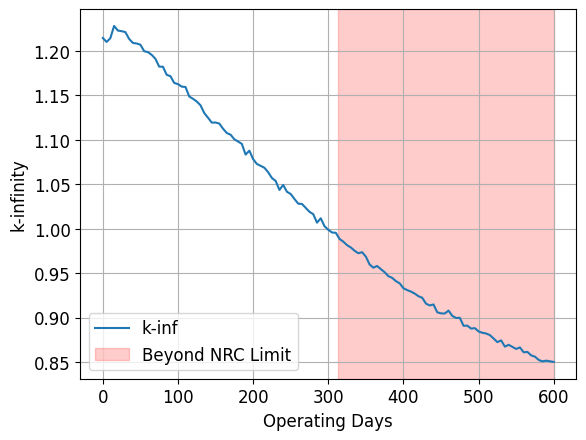
\includegraphics[width=0.8\linewidth]{figs/kinfVsBurn.png}
    \caption{Infinite multiplication factor $k_\infty$ versus accumulated burnup at 30\,W/gHM for the D$_2$O / 6\,cm pitch infinite lattice, starting from the TMI-1 C2B composition at 52.6\,GWd/tHM. Criticality is maintained through an additional 9.0\,GWd/tHM, reaching a total of $\sim$61.6\,GWd/tHM and exceeding the 60\,GWd/tHM design objective. The shaded region indicates operation beyond the NRC regulatory burnup ceiling of 62\,GWd/tHM.}
    \label{fig:kinf-burn}
\end{figure}

\paragraph{Fissile Inventory Evolution.}
The evolution of key fissile isotopes is shown in Figure~\ref{fig:conc-burn}. Over the 9.0\,GWd/tHM LBR irradiation, $^{235}$U depletes from 0.74\,wt\% to 0.30\,wt\% (a 59\% reduction), while $^{239}$Pu depletes from 0.59\,wt\% to 0.39\,wt\% (a 34\% reduction). Total plutonium decreases from 1.26\,wt\% to 0.99\,wt\%, a 21.5\% reduction that exceeds the 20\% design target. Continuous breeding from $^{238}$U partially replenishes the $^{239}$Pu inventory, consistent with the $\lambda_3/\lambda_2 > 1$ condition established earlier: net destruction proceeds, but is partially offset by in-situ production. Integrating over the full core, this corresponds to the destruction of approximately 16\,kg of plutonium per tonne of heavy metal processed, or $\sim$1\,070\,kg total.

\begin{figure}[H]
    \centering
    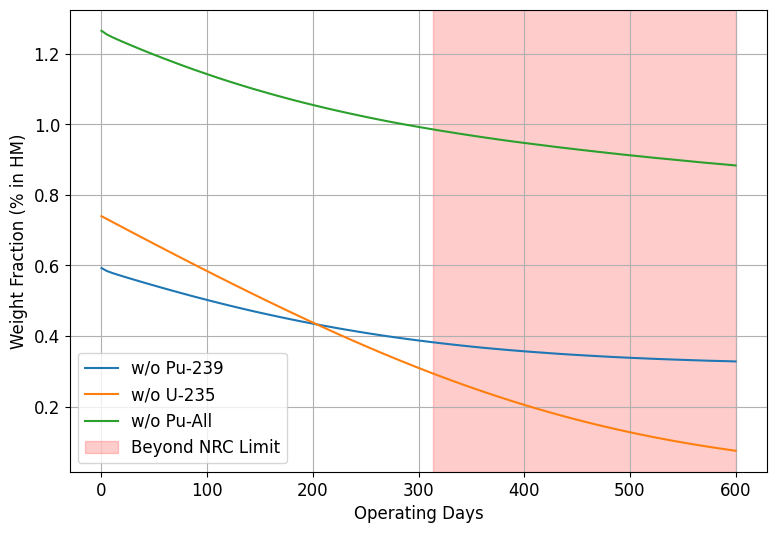
\includegraphics[width=0.8\linewidth]{figs/concVsBurn.png}
    \caption{Fissile isotope weight fractions versus operating time. $^{235}$U depletes from 0.74\% to 0.30\% (59\% reduction) while $^{239}$Pu depletes from 0.59\% to 0.39\% (34\% reduction). Total plutonium decreases from 1.26\% to 0.99\%, a 21.5\% reduction exceeding the 20\% design target. Continuous breeding from $^{238}$U partially replenishes the $^{239}$Pu inventory, consistent with the $\lambda_3/\lambda_2 > 1$ condition.}
    \label{fig:conc-burn}
\end{figure}

\paragraph{Plutonium Isotopic Quality Degradation.}
Beyond total mass reduction, the isotopic composition of the remaining plutonium evolves in a direction that degrades its weapons utility. As shown in Figure~\ref{fig:attractiveness}, the fissile isotopes $^{239}$Pu and $^{241}$Pu decrease over the cycle while $^{238}$Pu, $^{240}$Pu, and $^{242}$Pu accumulate. The relative $^{239}$Pu fraction decreases by 24.7\%, while the $^{240}$Pu fraction --- which carries a high spontaneous fission rate --- increases by 30.0\% relative to total plutonium. This isotopic shift simultaneously reduces net fissile content and increases self-heating and neutron emission rates, degrading the material's utility for weapons applications even if it were chemically separated.

\begin{figure}[H]
    \centering
    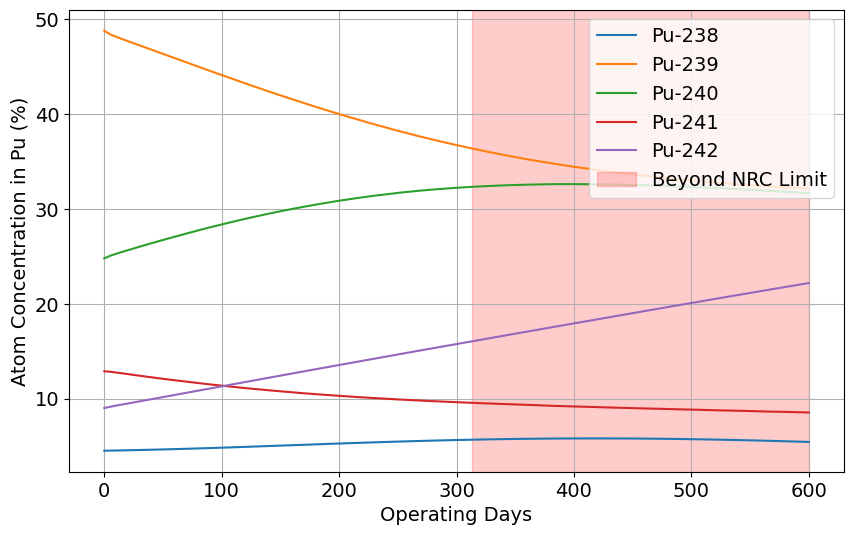
\includegraphics[width=0.8\linewidth]{figs/attractiveness.png}
    \caption{Plutonium isotopic composition versus operating time. The fissile isotopes $^{239}$Pu and $^{241}$Pu decrease while $^{238}$Pu, $^{240}$Pu, and $^{242}$Pu accumulate, progressively degrading weapons attractiveness through elevated decay heat, higher spontaneous fission rates, and a reduced fissile fraction.}
    \label{fig:attractiveness}
\end{figure}

\paragraph{0-D Scoping Summary.}
The 0-D infinite lattice analysis confirms that the two neutronics-driven design objectives are achievable at the scoping level:
\begin{itemize}
    \item \textbf{Objective 1 --- Plutonium reduction}: $^{239}$Pu decreases by 34\% and total Pu by 21.5\%, both exceeding the $\geq$20\% target; $^{240}$Pu fraction increases by 30\%, degrading weapons attractiveness.
    \item \textbf{Objective 2 --- Sustained criticality}: $k_\infty \geq 1$ through 9.0\,GWd/tHM of additional irradiation, reaching a total accumulated burnup of $\sim$61.6\,GWd/tHM and exceeding the $\geq$60\,GWd/tHM target.
\end{itemize}

These results assume spatially uniform depletion in an ideal infinite lattice. Several phenomena lie outside the scope of this approximation and require higher-fidelity treatment before the design can be considered credible:

\begin{enumerate}
    \item \textbf{Non-uniform spent fuel burnup.} Real PWR assemblies discharge with a spatially varying burnup profile: rod extremities retain substantially more fissile material than the axial midplane. A 0-D model assigns a single composition to the entire fuel volume and therefore cannot represent this variation, meaning the isotopic starting conditions for the LBR differ significantly from those of a single-composition infinite lattice.
    \item \textbf{Isotopic validation.} The 0-D model uses a single measured composition from SFCOMPO-2.0, but a full assembly model requires spatially varying fuel compositions across the rod length. These must be generated by a depletion code and subsequently validated against the remaining measured compositions in SFCOMPO-2.0 before they can be trusted as LBR fuel inputs.
    \item \textbf{Spectral coupling between moderator and fuel.} The spatial distribution of D$_2$O and fuel in a real assembly modifies both the effective moderation ratio and the flux-weighted cross sections relative to the infinite lattice assumption, altering the predicted reaction rate balance.
    \item \textbf{Axial power redistribution.} The non-uniform fissile profile drives an axially peaked power distribution that is invisible to 0-D models but directly affects cycle length, thermal margins, and fuel utilization efficiency.
\end{enumerate}

These limitations define the scope of the detailed Monte Carlo analyses presented in \S~\ref{sec:neutronics}: (i)~a Serpent~2 depletion model of Assembly NJ05YU from TMI-1 is benchmarked against measured isotopic data to validate the spent fuel compositions; (ii)~a full-assembly Serpent lattice model replaces the infinite lattice approximation for moderator and pitch selection; and (iii)~an iterative design study identifies and optimizes a power-redistribution strategy to address the axial burnup non-uniformity that the scoping analysis could not resolve.